\documentclass[11pt,a4paper,twoside]{article}
\usepackage[utf8]{inputenc}
\usepackage{polski}



\usepackage{graphicx}
\usepackage{subcaption} % obrazki obok siebie
%\usepackage[caption=false]{subfig} % obrazki nad sobą
\usepackage{wrapfig} 
\usepackage{float}
\usepackage{geometry}
%\geometry{lmargin=3cm,rmargin=2cm, tmargin=2.5cm, bmargin=2.5cm} %marginesy w pracy inż/mgr
\geometry{lmargin=2.5cm,rmargin=2.5cm, tmargin=2.5cm, bmargin=2.5cm} %marginesy ogólne
\usepackage{multirow} % scalanie wierszy tabeli

\usepackage{fancyhdr}
\pagestyle{fancy}
\fancyhead{} % wszystkie nagłówki puste
%\fancyhead[RE,LO]{ Absolwenci Wydziału Prawa  2012}
\fancyfoot{} % wszystkie stopki puste
\fancyfoot[LE,RO]{\thepage}
\renewcommand{\headrulewidth}{0pt}
%\renewcommand{\footrulewidth}{0.4pt}

\usepackage[hidelinks]{hyperref}% nazwy odsyłaczy

%unikanie myślników dzielących słowa między liniami
\tolerance=1
\emergencystretch=\maxdimen
\hyphenpenalty=10000
\hbadness=10000

\usepackage{algorithm}
\usepackage{algorithmicx}
\usepackage{algpseudocode}
\makeatletter
\renewcommand{\ALG@name}{Algorytm}
\renewcommand{\figurename}{Wykres}

\usepackage{enumitem}
\setitemize{itemsep=2pt,topsep=2pt,parsep=2pt,partopsep=2pt} %odstępy wyliczanych elementów (-)

\usepackage{indentfirst} % wcięcie w pierwszym akapicie (pod)rozdziału
%%%%%%%%%%%%%%%%%%%%%%%%%%%%%%%%%%%%%%%%% formatowanie kodu R
\usepackage{listings} 
\usepackage{color}
\definecolor{gray}{rgb}{0.5,0.5,0.5}
\lstset{
language=R,
basicstyle=\footnotesize\ttfamily,%\scriptsize\ttfamily,
commentstyle=\ttfamily\color{gray},
numbers=left,
numberstyle=\ttfamily\color{gray}\footnotesize,
stepnumber=0, % numeracja linii
numbersep=5pt,
backgroundcolor=\color{white},
showspaces=false,
showstringspaces=false,
showtabs=false,
frame=none, % obramowanie kodu
tabsize=2,
captionpos=b,
breaklines=true,
breakatwhitespace=false,
title=\lstname,
escapeinside={},
keywordstyle={},
morekeywords={}
}
%%%%%%%%%%%%%%%%%%%%%%%%%%%%%%%%%%%%%%%%%

%%% zawijanie tekstu w tabelach zgodnie z życzeniem
\usepackage{stackengine}
\usepackage{array}
\newcolumntype{L}[1]{>{\raggedright\arraybackslash}p{#1}}
\setstackEOL{\#}
\setstackgap{L}{12pt}
%%%

\usepackage{amsfonts} % zbiory liczba (np. naturalnych)
\usepackage{amsmath} %duże klamry
\usepackage{bbm} %skok jednostkowy
\usepackage[titletoc,title]{appendix} % dodatki - zmiana wyświetlania nagłówka
\pagenumbering{gobble}
\usepackage{afterpage} % pusta strona
\usepackage{tabularx}

\usepackage{makecell}

%\usepackage{setspace} % interlinia
%\singlespacing 
%\onehalfspacing
%\doublespacing
%\setstretch{0.96}

\begin{document}
\pagenumbering{arabic}
\begin{center}
\vspace*{3\baselineskip}
{\LARGE{MOW Projekt 13}}
\\
\vspace*{1\baselineskip}
{\large{Porównanie algorytmów grupowania i klasyfikacji do detekcji anomalii.}}
\\
\vspace*{1\baselineskip}
Katarzyna Piórkowska, 259078 \\
Tomasz Korzeniowski, 265753 \\
\vspace*{1\baselineskip}
\today
\end{center}
\section{Zadanie}
\subsection{Treść}
Nienadzorowana detekcja anomalii za pomocą odpowiednio opakowanych wybranych algorytmów grupowania dostępnych w R. Porównanie z nadzorowaną detekcją anomalii za pomocą dostępnych w R algorytmów klasyfikacji.
\subsection{Interpretacja}
W ramach projektu należy zbadać czy możliwe jest wykrycie anomalii w danych korzystając ze standardowych algorytmów grupowania dostępnych w R. W tym celu należy zapewnić mechanizm generowania modelu grupowania, który zwróci podział danych trenujących na grupy. Następnie, dla każdego nowego przykładu testowego, trzeba ocenić w jakim stopniu jest on podobny do którejś z wyznaczonych grup. Ocena polegać będzie na wyznaczeniu wskaźnika nietypowości, który jest miarą liczbową wskazującą na ile badany przykład jest niepodobny do rozważanych grup.

Do symulowania anomalii w danych przyjmiemy, że jedna z klas w nich występująca (np. najmniej liczna) będzie stanowiła anomalie. Przykłady należące do tej klasy nie zostaną wykorzystane do budowy modelu grupowania.

Częścią implementacji projektu będzie zapewnienie opakowania wybranych algorytmów grupowania w funkcję, która zwraca model pogrupowanych danych trenujących. Użytkownik będzie miał możliwość podania metody grupowania z jakiej chce skorzystać (wraz z jej niezbędnymi parametrami). Inna funkcja będzie miała za zadanie skorzystać z wyznaczonego modelu oraz dopasować dane testowe przez wyznaczenie zadanego wskaźnika nietypowości.

W części analitycznej zostanie przeprowadzona symulacja wykrywania anomalii na kilku zbiorach danych. Wyniki otrzymane przy użyciu zaimplementowanych funkcji zostaną porównane z wynikami uzyskanymi przez zastosowanie znanych algorytmów klasyfikacji dostępnych w R. W tym drugim przypadku algorytmy będą znały klasy do jakich należą obserwacje by wskazać anomalie jako jedną z klas. Porównanie wyników obu podejść będzie polegało na wyznaczeniu wskaźników jakości (dokładności) powyższych rozwiązań.

\section{Algorytmy}
Do realizacji zadania zostaną wykorzystane trzy algorytmy grupowania (k-średnich, k-medoidów, grupowania hierarchicznego) oraz dwie metody klasyfikacji (drzewa decyzyjne, k najbliższych sąsiadów). Każdy z nich zostanie pokrótce opisany wraz ze wskazaniem kluczowych parametrów.

\subsection{Algorytm k-średnich}
Algorytm k-średnich jest jednym z najprostszych algorytmów rozwiązujących zadanie grupowania. Ideą algorytmu jest przyporządkowanie pewnego zbioru \mbox{N przykładów} do przyjętej a priori liczby grup K. Każda grupa posiada dokładnie jeden centroid, czyli punkt reprezentujący wartość średnią grupy. Pojedynczą obserwację $x_{i} = (x_{1}, x_{2},\ldots, x_{N})$ można przyporządkować tylko do jednego z centroidów $c_{j} = (c_{1}, c_{2},\ldots, c_{K})$ Oznacza to minimalizację funkcji: \begin{equation}
J = \sum_{j=1}^{K}{\sum_{i=1}^{N} {\|x_{i}-c_{j}\|}^{2}}
\end{equation} Po zakończeniu pojedynczej iteracji grupowania należy uaktualnić położenie centroidów i przyporządkować obserwacje ponownie. Przebieg grupowania przedstawia algorytm \ref{kMeans}.
\begin{algorithm}[ht]
\caption{k-średnich}
\label{kMeans}
	\begin{algorithmic}%[1]
	\State{1. Wyznacz początkowe położenie centroidów}
	\State{2. Przyporządkuj każdej obserwacji najbliższy jej centroid.}
	\State{3. Gdy wszystkie obserwacje zostaną przyporządkowane, wyznacz ponownie położenie centroidów, znajdując wartość średnią obserwacji przypisanych do centroidu: $$c_{ji}=\frac{1}{M}\sum_{m=1}^{M} {x_{m}} \quad ,gdzie \ M - liczba \ obserwacji \ w \ c_{j}$$}
	\State{4. Powtarzaj kroki 2. i 3., dopóki centroidy zmieniają swoje położenie lub nie zostanie osiągnięta maksymalna liczba iteracji.}
	\end{algorithmic}
\end{algorithm}

Do zalet algorytmu należy proste znajdowanie podziału grup dobrze odseparowanych od siebie. Największą wadą algorytmu jest konieczność podania liczby grup na jakie chcemy podzielić dane. Ponadto początkowe położenie centroidów determinuje wynik grupowania. Algorytm nie radzi sobie również z danymi silnie zaszumionymi i/lub zawierającymi obserwacje odstające (zaburzenie średniej). 

W środowisku R istnieje funkcja \textit{kmeans} w standardowym pakiecie \textit{stats}, która realizuje algorytm k-średnich.
\begin{verbatim}
kmeans(x, centers, iter.max = 10, nstart = 1,
       algorithm = c("Hartigan-Wong", "Lloyd", "Forgy",
                     "MacQueen"), trace=FALSE)
\end{verbatim}

Jej główne parametry wejściowe to:
\begin{table}[ht]
%\caption{Rejestr zmian}
\label{etapyProjektu}
\centering
\begin{tabularx}{\textwidth}{lcX}
 x & -- & zbiór danych (numerycznych) do pogrupowania \\
 centers & -- & wstępne położenie centroidów lub ich liczba oznaczająca na jak wiele grup należy podzielić dane \\
 iter.max & -- & maksymalna liczba iteracji algorytmu, warunek stopu\\
\end{tabularx}
\end{table}

Pozostałe parametry związane są z wewnętrzną implementacją algorytmu w pakiecie R i nie będą rozpatrywane w ramach projektu. Wynikiem działania algorytmu jest model zawierający wektor przyporządkowania obserwacji do grup, środki wyznaczonych grup oraz pomocnicze miary (suma kwadratów odległości między przykładami w grupie, liczność grup, liczba wykonanych iteracji)

\subsection{Algorytm k-medoidów}
Struktura algorytmu k-medoidów jest niemal taka sama jak algorytmu k-średnich. Jedną różnicą jest przyjęcie, że środkiem grupy jest medoid, a nie wartość średnia. Medoid jest najbardziej centralnym przykładem w grupie (średnia grupy może się nie pokrywać z żadnym przykładem należącym do wyznaczonej grupy). Powoduje to uodpornienie algorytmu na wartości odstające.

Aby wybrać nowy medoid, w kolejnych iteracjach algorytmu, rozważane są wszystkie przykłady $p$. Istnieją 4 możliwe przypadki, które należy sprawdzić by stwierdzić czy przykład $p$ (niebędący medoidem) może zastąpić medoid $m$:

\begin{enumerate}
\item Przykład $a$ należy do grupy medoidu $m$ -- jeśli zastąpimy $m$ przykładem $p$ oraz $a$ znajduje się bliżej medoidu $n$ to przydziel $a$ do grupy $n$.
\item Przykład $a$ należy do grupy medoidu $m$ -- jeśli zastąpimy $m$ przykładem $p$ oraz $a$ znajduje się bliżej przykładu $p$ to przydziel $a$ do nowego medoidu $p$.
\item Przykład $a$ należy do grupy medoidu $n$ -- jeśli zastąpimy medoid $m$ przykładem $p$ oraz $a$ znajduje się bliżej medoidu $n$ to nie zmieniaj przydziału przykładu $a$.
\item Przykład $a$ należy do grupy medoidu $n$ -- jeśli zastąpimy medoid $m$ przykładem $p$ oraz $a$ znajduje się bliżej $p$ to przydziel $a$ do nowego medoidu $p$.
\end{enumerate}

Powyższe możliwości ilustruje wykres \ref{kMedoidsSwap}.

\begin{figure}[ht]
%\vspace{-20pt}
\centering
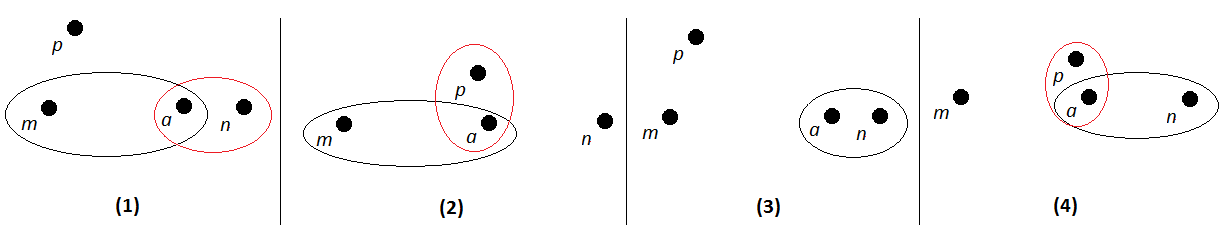
\includegraphics[height=3cm, width=15.7cm]{kMedoids2}
\caption{Przypadki zamiany medoidu $m$ przykładem $p$.}
\label{kMedoidsSwap}
\end{figure}

Przebieg grupowania przedstawia algorytm \ref{kMedoids}.

\begin{algorithm}[ht]
\caption{k-medoidów}
\label{kMedoids}
	\begin{algorithmic}%[1]
	\State{1. Wybierz $K$ przykładów jako medoidy.}
	\State{2. Przyporządkuj każdej obserwacji najbliższy jej medoid.}
	\State{3. Dla każdego medoidu $m$ wybierz inny przykład $p$, który zmniejszy odległość między przykładami w obrębie nowej grupy.}
	\State{4. Powtarzaj kroki 2. i 3., dopóki medoidy zmieniają się lub nie zostanie osiągnięta maksymalna liczba iteracji.}
	\end{algorithmic}
\end{algorithm}

W języku R istnieje algorytm $pam$ (ang. partitioning around medoids) w pakiecie cluster, który implementuje algorytm k-medoidów.

\begin{verbatim}
pam(x, k, diss = inherits(x, "dist"), metric = "euclidean",
    medoids = NULL, stand = FALSE, cluster.only = FALSE, do.swap = TRUE,
    keep.diss = !diss && !cluster.only && n < 100,
    keep.data = !diss && !cluster.only, pamonce = FALSE, trace.lev = 0)
\end{verbatim} 

Najważniejsze parametry wejściowe to:

\begin{table}[H]
\label{kMedoids_params}
\centering
\begin{tabularx}{\textwidth}{lcX}
 x & -- & zbiór danych (numerycznych) do pogrupowania \\
 k & -- & docelowa liczba grup \\
metric & -- & metryka, według której obliczana jest odległość \\
stand & -- & flaga binarna określająca czy dane mają być standaryzowane \\
\end{tabularx}
\end{table}

W wyniku działania algorytmu otrzymujemy klasę, która zawiera informacje o wyznaczonych medoidach oraz przydział grupy dla każdego przykładu. Ponadto można znaleźć informację o miarach odległości między obserwacjami.

\subsection{Algorytm hierarchiczny}
Algorytmy hierarchiczne pozwalają na graficzną reprezentację struktury klasteryzacji w postaci drzewa. Można wyróżnić tu dwa podejścia: aglomeracyjne, gdzie każda z obserwacji stanowi na początku oddzielną grupę oraz partycjonujące - rozpoczynające od jednej grupy zawierającej wszystkie próbki. Przebieg aglomeracji przedstawia algorytm \ref{hierarch}.

\begin{algorithm}[ht]
\caption{hierarchiczny}
\label{hierarch}
	\begin{algorithmic}
	\State{1. Utwórz jednoelementowe grupy.}
	\State{2. Zbuduj macierz odległości pomiędzy rozpatrywanymi elementami.}
	\State{3. Znajdź parę elementów, między którymi odległość jest najmniejsza.}
	\State{4. Połącz znalezione grupy w jedną i wyznacz ich nowy środek ciężkości jako średnią środków cieżkości grup składowych.}
	\State{5. Powtarzaj kroki 2-4 aż do uzyskania jednego skupiska zawierającego wszystkie próbki.}
	\end{algorithmic}
\end{algorithm}

Do zalet algorytmów hierarchicznych należy brak konieczności początkowego określenia liczby klas w przeciwieństwie do opisanych wyżej algorytmów k-średnich i k-medoidów. Do wad można zaliczyć dość duże zróżnicowanie wyników w zależności od wybranych metod łączenia grup, wśród których znajdują się m.in. metody najbliższych i najdalszych sąsiadów, metoda średnich (centroidów) oraz minimalnej wariancji Warda.

Algorytmem aglomeracyjnym dostępnym w języku R jest agnes (ang. agglomerative nesting) w pakiecie cluster.

\begin{verbatim}
agnes(x, diss = inherits(x, "dist"), metric = "euclidean",
      stand = FALSE, method = "average", par.method,
      keep.diss = n < 100, keep.data = !diss, trace.lev = 0)
\end{verbatim} 

Jego najważniejsze parametry wejściowe to:

\begin{table}[ht]
\label{agnes_params}
\centering
\begin{tabularx}{\textwidth}{lcX}
 x & -- & zbiór danych (numerycznych) do pogrupowania \\
metric & -- & metryka, według której obliczana jest odległość \\
method & -- & metoda łączenia grup\\
\end{tabularx}
\end{table}

Wynikiem działania algorytmu jest graficzna reprezentacja struktury grupowania - dendrogram. Ponadto obliczany jest współczynnik aglomeracji, który charakteryzuje wygląd dendrogramu: niski współczynnik oznacza węższe struktury.

\subsection{Drzewa decyzyjne}

Pierwszą z metod klasyfikacji stosowaną w celu porównania z algorytmami grupowania są drzewa decyzyjne. W języku R istnieje wiele jej implementacji, z których wykorzystany zostanie algorytm C4.5 przedstawiony poniżej.

\begin{algorithm}[H]
\caption{Algorytm C4.5}
\label{decision_tree}
	\begin{algorithmic}
	\State{1. Utwórz zbiór treningowy T.}
	\State{2. Wybierz taki atrybut, który najlepiej różnicowałby przykłady ze zbioru T.}
	\State{3. Utwórz węzeł drzewa odpowiadający wybranemu atrybutowi.}
	\State{4. Do węzła dodaj podwęzły, z których każdy reprezentuje pewną wartość badanego atrybutu.}
	\State{5. Powtarzaj podziały dla kolejnych podwęzłów.}
	\end{algorithmic}
\end{algorithm}

Do niewątpliwych zalet drzew decyzyjnych należy czytelna forma reprezentacji, efektywność pamięciowa oraz wszechstronność metody. Konieczny jest w niej jednak kompromis pomiędzy wielkością drzewa a jakością klasyfikacji. Drzewa mogą być również podatne na zjawisko nadmiernego dopasowania.

Wykorzystaną w projekcie funkcją będzie J48 z pakietu RWeka.

\begin{verbatim}
J48(formula, data, subset, na.action,
    control = Weka_control(), options = NULL)
\end{verbatim} 

Jego najważniejsze parametry wejściowe to:

\begin{table}[ht]
\label{j48_params}
\centering
\begin{tabularx}{\textwidth}{lcX}
formula & -- & symboliczny opis modelu \\
data & -- & dane treningowe \\
\end{tabularx}
\end{table}

Wynikiem działania funkcji jest schemat drzewa decyzyjnego wraz z opisem jego węzłów oraz dane o jego wielkości.

\subsection{Metoda k najbliższych sąsiadów}

Metoda k najbliższych sąsiadów zaliczana jest do grupy algorytmów tzw. leniwego uczenia. Nie tworzy ona żadnej reprezentacji danych w postaci modelu, a szuka rozwiązania dopiero w momencie pojawienia się przykładu do klasyfikacji. Aby zastosować metodę najbliższego sąsiada konieczne jest przedstawienie obiektów w n-wymiarowej przestrzeni po czym umieszczenie w niej obiektu testowanego. Klasyfikacja sprowadza się do sprawdzenia, do jakiej klasy należy obiekt najbliższy obiektowi testowanemu. Jeżeli wybrany został wariant metody z k sąsiadów to najpierw konieczne jest rozstrzygnięcie, która klasa dominuje wśród nich.

\begin{algorithm}[ht]
\caption{Algorytm k najbliższych sąsiadów}
\label{kNN}
	\begin{algorithmic}
	\State{1. Oblicz odległości klasyfikowanego przykładu od przykładów ze zbioru treningowego.}
	\State{2. Znajdź k najbliższych sąsiadów.}
	\State{3. Sklasyfikuj przykład na podstawie klas sąsiadów.}
	\end{algorithmic}
\end{algorithm}

Podstawową zaletą algorytmu kNN jest jego prostota. Ma on jednak szereg wad, do których należy długi czas obliczeń w przypadku licznych zbiorów treningowych, duże wymagi pamięciowe oraz konieczność wstępnej normalizacji danych. Język R oferuje tutaj funkcję kNN.

\begin{verbatim}
knn(train, test, cl, k = 1, prob = FALSE, 
algorithm=c("kd_tree", "cover_tree", "brute"))
\end{verbatim} 

Jego najważniejsze parametry wejściowe to:

\begin{table}[H]
\label{kNN_params}
\centering
\begin{tabularx}{\textwidth}{lcX}
train & -- & zbiór trenujący \\
test & -- & zbiór danych testowych \\
cl & -- & prawdziwe klasy, do których należą przykłady zbiory trenującego \\
k & -- & liczba sąsiadów \\
\end{tabularx}
\end{table}

%\newpage
\section{Opis badań}
\subsection{Planowane eksperymenty}

W projekcie przeprowadzone zostaną następujące eksperymenty:

\begin{enumerate}
  \item detekcja anomalii przy wykorzystaniu różnych wskaźników nietypowości dla różnych metod grupowania,
  \item porównanie grupowania z klasyfikacją za pomocą drzew decyzyjnych,
  \item porównanie grupowania z klasyfikacja za pomocą metody k najbliższych sąsiadów.
\end{enumerate}

%dokładność dla różnych danych - czy któryś z wybranych algorytmów jest lepszy od innych, czy lepsze jest grupowanie czy klasyfikacja
%miary nieprawidłowości z artykułu zamiast standardowych odległości przy badaniu danych testowych

W celu stwierdzenia czy testowany przykład należy zaliczyć do jednej z wyznaczonych grup czy też oznaczyć go jako anomalię wykorzystamy niestandardowe wskaźniki omówione w \cite{miaryNietypowosci}.

%W celu oceny anomalii konieczne jest użycie niestandardowych wskaźników, które nie tylko stwierdzą ich obecność, ale również określą ich właściwości. 

Pierwszym z proponowanych wskaźników jest CBLOF liczony jako iloczyn odległości $d$ badanej próbki $p$ od najbliższej dużej grupy ($C \in LC$) i liczby elementów w grupie, do której obiekt został zaklasyfikowany. Koncepcja małych (SC) i dużych (LC) grup nie jest precyzyjnie określona - możliwy jest wybór algorytmu podziału.
\begin{equation}
CBLOF(p) = \begin{cases}
   |C_{i}| \cdot min(d(p,C_{j})), & \text{jeśli}\ C_{i} \in SC \text{, gdzie } p \in C_{i} \text{ oraz } C_{j} \in LC\\
    |C_{i}| \cdot d(p,C_{j}), & \text{jeśli}\ C_{i} \in LC \text{, gdzie } p \in C_{i}
  \end{cases}
\end{equation}

Wskaźnik ten powinien rosnąć wraz z odległością próbki od dużej grupy, a zatem wskazywać na stopień anomali - im wyższa jego wartość, tym obiekt bardziej oddalony od grup. Jednak ze względu na fakt, że uwzględniana jest w nim również liczność grupy algorytm ten może dawać nieprawidłowe wyniki. Jako anomalie mogą zostać zaklasyfikowane próbki znajdujące się blisko bardzo licznych zbiorów.

Lepszym rozwiązaniem może być zatem nieważony wskaźnik CBLOF oparty jedynie na odległości od grup, z pominięciem ich liczności. W projekcie zostaną zastosowane obie wersje ocen anomalii i wykonane zostanie porównanie między nimi.

\begin{equation}
u-CBLOF(p) = \begin{cases}
   min(d(p,C_{j})), & \text{jeśli}\ p \in SC \text{, gdzie } C_{j} \in LC\\
    d(p,C_{i}), & \text{jeśli}\ p \in C_{i} \in LC
  \end{cases}
\end{equation}

Inną miarą oceny anomalii jest LDCOF charakteryzująca się normalizacją wyników dla próbki względem jej sąsiedztwa. Definiowana jest jako iloraz odległości próbki od najbliższej dużej grupy i średniego dystansu między elementami tej dużej grupy i jej środkiem.

\begin{equation}
distance_{avg}(C) = \frac{\sum_{i \in C} d(i,C)}{|C|}
\end{equation}

\begin{equation}
LDCOF(p) = \begin{cases}
   \frac{min(d(p,C_{j}))}{distance_{avg}(C_{j}}, & \text{jeśli}\ p \in C_{i} \in SC \text{, gdzie } C_{j} \in LC\\
    \frac{d(p,C_{j})}{distance_{avg}(C_{j}}, & \text{jeśli}\ p \in C_{i} \in LC
  \end{cases}
\end{equation}

%czas wykonania?

\subsection{Zbiory danych}
%wybór atrybutów przed dokonaniem grupowania (możliwe ograniczenie do mniejszego podzbioru z uzasadnieniem), wstępne%przetwarzanie (funkcje tworzące model i klasyfikujące nie muszą same robić przekształceń)
%atrybuty brakujące (NA) - sposób w jaki będziemy sobie z nimi radzić
%decyzja o atrybucie klasy (np. ostatni atrybut)
%przekształcenie na dane numeryczne już we własnej funkcji
%opis wybranych zbiorów danych

Badania przeprowadzone zostaną na kilku zbiorach danych o numerycznych typach atrybutów. Wynika to z parametrów przyjmowanych przez wybrane algorytmy grupowania. Nie oznacza to jednak, że nie można grupować atrybutów dyskretnych. Wymagałoby to ich przewartościowania na wartości numeryczne.

Dla wszystkich zbiorów danych konieczne będzie określenie sposobu postępowania z brakującymi wartościami. W przypadku pojedynczych braków pewne próbki zostaną najprawdopodobniej pominięte lub też zastąpione średnią wartością atrybutu. Jeżeli brakujących wartości byłoby więcej, lepsze wyniki dałaby predykcja danej wartości.

Wstępne przetwarzanie atrybutów będzie odbywać się przed dostarczeniem danych do metody wyznaczającej grupowanie. Możliwe będzie również ograniczenie liczby wykorzystanych atrybutów. Klasyfikator k najbliższych sąsiadów będzie z kolei prawdopodobnie wymagał normalizacji danych. 

Wykorzystane zostaną przykładowe zbiory danych pochodzące z UCI Machine Learning Repository:
\begin{itemize}
\item Letter Recognition Data Set -- zbiór danych dotyczących zdjęć liter alfabetu,  zawiera 16 atrybutów oraz 26 klas
\item Mushroom Data Set -- zbiór danych opisujących grzyby. Możliwe są dwie klasy - grzyby jadalne lub trujące, zawiera 22 atrybuty
\item Dataset for Sensorless Drive Diagnosis Data Set -- zbiór danych diagnostycznych dla napędów komputerowych, możliwość klasyfikacji na podstawie 49 atrybutów do 11 klas
  %\item Gas sensor array under dynamic gas mixtures Data Set - zbiór danych z sensorów chemicznych,
  %\item Grammatical Facial Expressions Data Set - zbiór służący interpretacji mimiki na podstawie języka migowego,
  %\item Image Segmentation Data Set - segmentacja obrazów,
  %\item Mice Protein Expression Data Set - ekspresja białek mierzona w korze mózgu myszy,
  %\item TV News Channel Commercial Detection Dataset Data Set - zbiór cech audiowizualnych reklam.
\end{itemize}

\subsection{Ocena jakości}
Aby ocenić jakość rozwiązania trzeba sprawdzić skuteczność algorytmów. Do tego budowana będzie macierz pomyłek. W jej wierszach znajdują się klasy oryginalne do których należały obiekty, a w kolumnach klasy przewidziane. Na przecięciu wstawiana jest liczba obiektów poprawnie lub niepoprawnie sklasyfikowanych. 

W przypadku binarnym rozważmy dwie klasy: pozytywną i negatywną. Do klasy pozytywnej będziemy zaliczali wszystkie przykłady zaliczone do swoich prawdziwych grup, a do klasy negatywnej obserwacje stanowiące anomalie. W sytuacji, gdy pewna pozytywna obserwacja zostanie zaklasyfikowana jako negatywna lub odwrotnie, korzystamy z tabeli \ref{confusionMatrix}. Przynależność do klasy rzeczywistej oznacza faktyczną klasyfikację obserwacji do jednej z klas, a wynik klasyfikacji to decyzja o przynależności podjęta przez algorytm. Możliwe wyniki to:
\begin{itemize}[label={--}]
\item TP (ang. \emph{true positive}) -- poprawne zaklasyfikowanie do rzeczywistej grupy
\item FN (ang. \emph{false negative}) -- błędne zaklasyfikowanie przykładu (jako anomalii) do klasy negatywnej, gdy tak naprawdę należy do jednej ze znalezionych grup
\item FP (ang. \emph{false positive}) -- błędne zaklasyfikowanie obserwacji (do jednej ze znalezionych grup) do klasy pozytywnej, gdy tak naprawdę są to anomalie
\item TN (ang. \emph{true negative}) -- poprawne wykrycie anomalii
\end{itemize}

\begin{table}[ht]
\centering
\caption{Macierz pomyłek}
\label{confusionMatrix}
\begin{tabular}{|*{4}{c|}}
\cline{3-4}
  \multicolumn{2}{c}{} & \multicolumn{2}{|c|}{wynik klasyfikacji}\\\cline{3-4}
  \multicolumn{2}{c|}{} & pozytywna & negatywna\\\hline
  \multirow{2}{*}{klasa rzeczywista}& pozytywna & TP & FN\\\cline{2-4}
  & negatywna & FP & TN\\\hline
\end{tabular}
\end{table}

Na tej podstawie można wyznaczyć wskaźniki jakości rozwiązania:
\begin{itemize}[label={--}]
\item dokładność -- liczba poprawnie sklasyfikowanych obserwacji wśród wszystkich wyników klasyfikacji $$\text{\emph{dokładność}} = \frac{TP+TN}{TP+TN+FP+FN}$$
\item precyzja -- liczba poprawnie sklasyfikowanych przykładów wśród wszystkich obserwacji zaklasyfikowanych do znalezionych grup $$\text{\emph{precyzja}} = \frac{TP}{TP+FP}$$
\end{itemize}

%W przypadku większej liczby klas, macierz pomyłek wyznaczana będzie korzystając z podejścia OVA.

\section{Kwestie otwarte}
W chwili pisania niniejszego sprawozdania nie przewidujemy zmiany domyślnych parametrów algorytmów, które nie są bezpośrednio związane z zadaniem (np. wybór implementacji algorytmu k-średnich w ramach funkcji \textit{kmeans}). Jeśli podczas testów okaże się, że pewne parametry nieomówione powyżej będą zmieniane, zostanie podana stosowna adnotacja.

Do oceny jakości klasyfikacji zostały wybrane wskaźniki dokładności i precyzji. W sytuacji gdy wskaźniki te nie będą w stanie wystarczająco jednoznacznie wyznaczyć, które z rozwiązań jest lepsze, zostaną rozważone i opisane inne miary jakości.

\begin{thebibliography}{9}
%\addcontentsline{toc}{section}{Literatura}
%\bibitem{BOCD}
%Z. Michalewicz, D. B. Fogel
%\emph{Jak to rozwiązać czyli nowoczesna heurystyka}.
%WNT, Warszawa 2006
\bibitem{k-methods}
\url{http://wazniak.mimuw.edu.pl/images/8/86/ED-4.2-m11-1.01.pdf}
\bibitem{miaryNietypowosci}
\url{https://www.goldiges.de/publications/Anomaly_Detection_Algorithms_for_RapidMiner.pdf}
\bibitem{drzewaDecyzyjne}
\url{https://www.mimuw.edu.pl/~awojna/SID/referaty/strzelczak/c4_5Main.html}
\bibitem{kSasiadow}
\url{https://edu.pjwstk.edu.pl/wyklady/adn/scb/wyklad9/w9.htm}
\bibitem{kSasiadow}
\url{https://www.rdocumentation.org/}

%\bibitem{knapsack3}
%\url{http://home.agh.edu.pl/~slukasik/pub/021_Lukasik_KAEiOG2011(presentation).pdf}
%\bibitem{knapsack4}
%\url{https://eti.pg.edu.pl/documents/176546/25263566/SZ_wyklad2.pdf}

\end{thebibliography}

\end{document}